\chapter{Strongest-alternative matched comparison}
\label{STC-S08}

이 장은 ``아무 기억도 없는 fixed model''이 아니라 문제별 strongest plausible alternative와 STC를
matched total work, state, quality, governance에서 비교한다. Sleep phase의 장점이 transform algorithm
자체의 장점인지 scheduling/validation의 장점인지도 분리한다.

\section{비교 원칙}

\begin{enumerate}
  \item 같은 base model, wake trace, validation set, hardware budget을 사용한다.
  \item external index build와 parametric training의 ingest·validation·publish 비용을 모두 포함한다.
  \item per-query 비용은 같은 future query trace에서 측정하고 one-time cost와 분리한다.
  \item capacity budget을 맞추고 old/new/safety/delete slice를 여러 sleep cycle에 걸쳐 평가한다.
  \item source-of-truth, rollback, base-version change를 operational metric으로 포함한다.
\end{enumerate}

\section{문제별 matched baseline}

\begin{longtable}{p{0.16\textwidth} p{0.22\textwidth} p{0.24\textwidth} p{0.27\textwidth}}
\caption{문제별 strongest non-STC baseline과 조건부 verdict}\label{tab:matched-alternatives}\\
\toprule
Problem & Strongest baseline & STC candidate & Conditional verdict \\
\midrule
\endfirsthead
\toprule
Problem & Strongest baseline & STC candidate & Conditional verdict \\
\midrule
\endhead
\midrule\multicolumn{4}{r}{다음 쪽에 계속}\\
\endfoot
\bottomrule
\endlastfoot
one-off long document & long-context inference & compile/summarize before query & reuse 없으면 baseline 우세 \\
repeated corpus QA & RAG + cache & background index/summary/latent compile & valid query reuse가 break-even 초과 시 STC 가능 \\
mutable factual memory & temporal RAG/graph & scheduled conflict resolution & destination은 external sleep 우세 \\
stable user preference & profile retrieval & user adapter promotion & high reuse·low churn·easy rollback에서 parametric 후보 \\
rare correction & ROME/MEMIT or record edit & sleep batch edit/replay & immediate edit 우세, sleep은 multi-edit integration \\
continual skill & replay+PEFT/global refresh & per-domain consolidation & bounded state에서 retention 입증 시 후보 \\
agent strategy & reflection/ReasoningBank & multi-episode strategy synthesis & external sleep evidence가 강함 \\
serving efficiency & prefix/state cache & sleep state compaction & state reuse와 compatibility가 높을 때만 \\
global knowledge & scheduled continued PT & wake-derived global sleep queue & 이름보다 cadence·data quality 비교 \\
privacy-local adaptation & on-device profile/RAG & on-device LoRA/compaction & thermal/endurance 포함한 matched test 필요 \\
\end{longtable}

\section{Hybrid recommendation}

\begin{figure}[htbp]
  \centering
  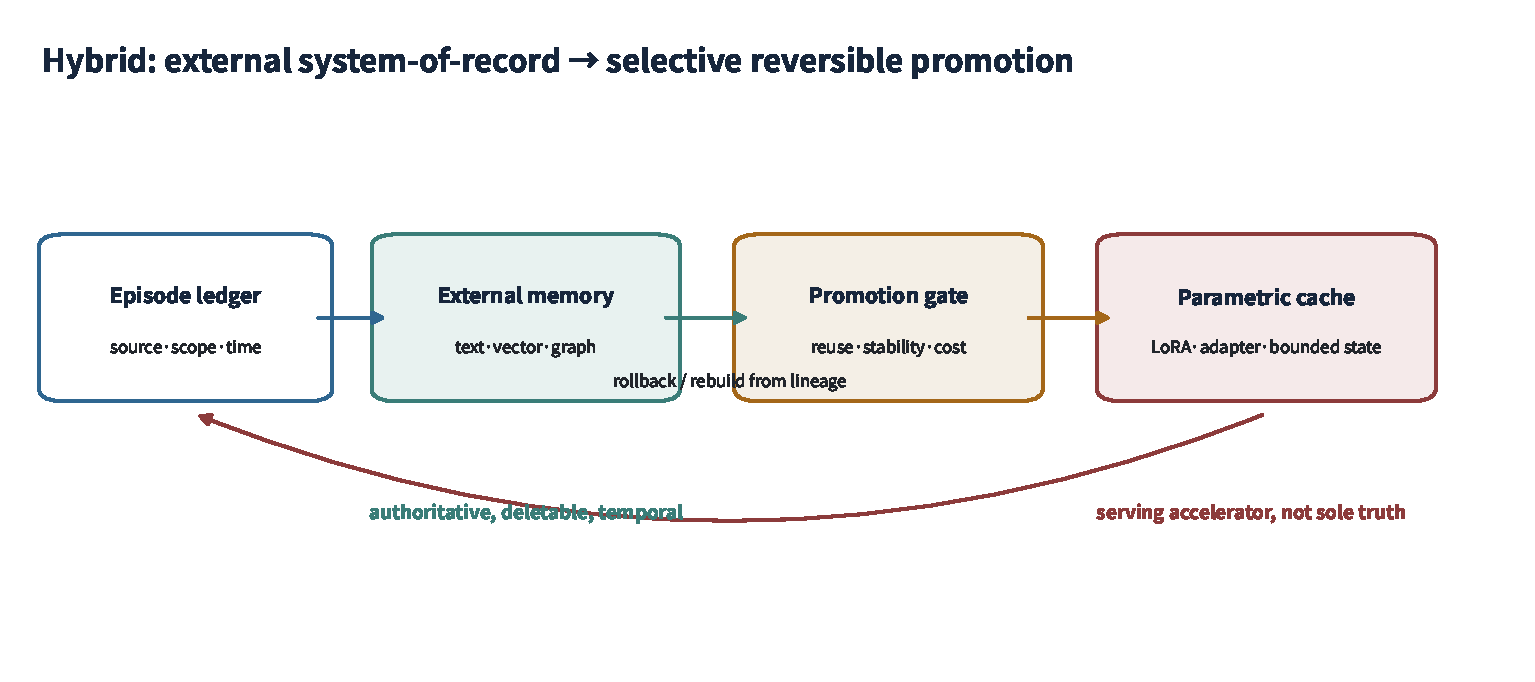
\includegraphics[width=0.98\textwidth]{figures/stc-f006.pdf}
  \caption{External system-of-record와 selective reversible parametric promotion. External evidence plane은
  authoritative하고, parametric state는 break-even을 통과한 serving cache로 취급한다.}
  \stcfigure{STC-F006}
  \figsource{Original synthesis; SRC-STC-0030, SRC-STC-0066}{Episode ledger가 external text-vector-graph memory와 promotion gate를 지나 LoRA-adapter cache로 이어지고 rollback은 provenance를 따라 원점으로 돌아가는 구조.}
  \label{fig:hybrid-promotion}
\end{figure}

Hybrid는 항상 절충안이라서 선택하는 것이 아니다. 서로 다른 content class가 요구하는 property가 다르기
때문이다. Changing fact와 rights-sensitive episode는 external source-of-record에 남고, repeated stable
behavior와 procedure는 adapter 또는 bounded neural state로 승격할 수 있다. 승격 뒤에도 original evidence를
남겨 rebase, delete, audit가 가능해야 한다.

Promotion score의 예는 다음과 같다.

\begin{equation}
P(e)=\alpha\,Reuse(e)+\beta\,Stability(e)+\gamma\,WakeSaving(e)
-\delta\,DeleteRisk(e)-\eta\,Interference(e)-\zeta\,RebaseCost(e).
\end{equation}

이는 학습된 universal score가 아니라 측정 항목을 빠뜨리지 않는 policy template다. Threshold는 user,
tenant, device, content class별로 다르며 uncertainty가 크면 external에 남긴다.

\section{STC가 이기지 못하는 영역}

\begin{itemize}
  \item 한 번만 읽는 document와 즉시 답이 필요한 query,
  \item 빠르게 변하고 exact citation·history·delete가 중요한 fact,
  \item future query distribution이 예측 불가능한 low-reuse memory,
  \item base model churn이 adapter lifetime보다 짧은 service,
  \item sleep candidate를 검증할 held-out trace가 없는 초기 product,
  \item state migration이 compute saving보다 큰 disaggregated infrastructure.
\end{itemize}

\begin{keypoint}[가장 강한 현재 판단]
External-memory sleep은 retrieval의 대체라기보다 writer·compactor·conflict resolver를 background로
옮기는 발전이다. Parametric sleep은 external system보다 본질적으로 더 긴 기억이 아니라, 반복되는
stable pattern의 serving cost를 선불로 지불하는 optimization이다.
\end{keypoint}
